\documentclass[a4paper]{article}

\usepackage[english]{babel}
\usepackage[utf8]{inputenc}
\usepackage{amsmath}
\usepackage{graphicx}
\usepackage[colorinlistoftodos]{todonotes}

\title{A Comparison between AMCMC and MCINTYRE}

\author{Your names and group number}

\date{\today}

\begin{document}
\maketitle

\begin{abstract}
% Enter a short summary here. What topic do you want to investigate and why? What experiment did you perform? What were your main results and conclusion?
\end{abstract}

\section{Introduction 5 lines to max 1/2 page}
\label{sec:introduction}

Explain the context of the experiment here. Why is condensed matter physics interesting or important?
Optional things you could talk about (but don't have to -- this is up to you): transistors, computers, Quantum computers, fundamental knowledge (e.g. the resistance quantum).

Briefly explain what methods you will use in the experiment, and what values you will extract from the data.

For this section and all following sections: If you refer to an equation, previous result or theory that is not regarded as common knowledge, then cite the source (article or book) where you found this. For example, you can cite the Nano 3 Lecture notes \cite{nano3}.

\section{Theory 2-3 pages}
\label{sec:theory}

%\subsection{Two-dimensional Electron Gas}
%Here, explain the concept of a 2-DEG in GaAs/AlGaAs. What is a 2-DEG and why does it arise?

%\subsection{Hall Effect}
%Explain the classical Hall effect in your own words. What do I measure at $B=0$? And what happens if $B>0$? Which effect gives rise to the voltage drop in the vertical direction?

%\subsection{Quantum Hall Effect}
%Explain the IQHE in your own words. What does the density of states look like in a 2-DEG when $B=0$? What are Landau levels and how do they arise? What are edge states? What does the electron transport look like when you change the magnetic field? What do you expect to measure?

\section{Experiment 1-2 pages}
\begin{itemize}
\item Purpose: running time comparison between AMCMC and MCINTYRE algorithms on 
      equivalent problems.
\item Experiments: every experiment is repeated on a different processor 
      thread. The results of these experiments are grouped by sample size so 
      it is possible to compute the average running times and standard 
      deviations.
\end{itemize}

\subsection{Fabrication}
%Explain a step-by-step recipe for fabrication here. How long did you etch and why? What is an Ohmic contact?
Explain the prolog code and the shell scripts.
\begin{itemize}
\item Once the data is saved on a CSV file the statistical computations and 
      plotting is respectively done by Numpy and Matplotlib.
\end{itemize}

\subsection{Experimental set-up}
% Explain the experimental set-up here. Use a schematic picture (make it yourself in photoshop, paint, ...) to show how the components are connected. Briefly explain how a lock-in amplifier works.
\begin{itemize}
    \item Hardware specs
    \item Software specs
\end{itemize}

\section{Results and interpretation 2-3 pages}

\begin{figure}
\centering
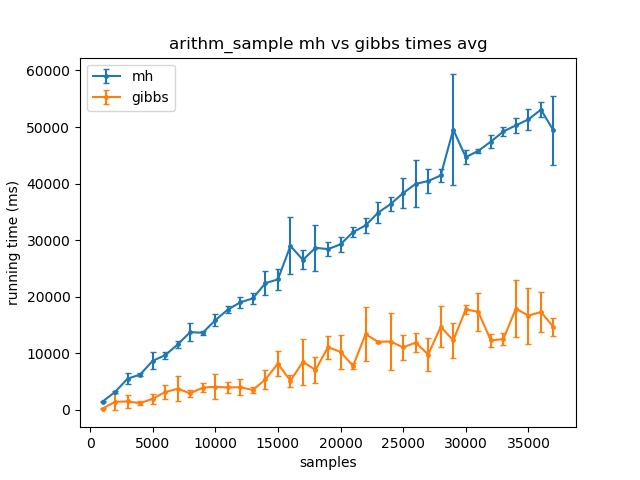
\includegraphics[width=1\textwidth]{plot_arithm_sample_mh_vs_gibbs_times.png}
\caption{\label{fig:data}Comparison between MH and Gibbs methods.}
\end{figure}

\begin{figure}
\centering
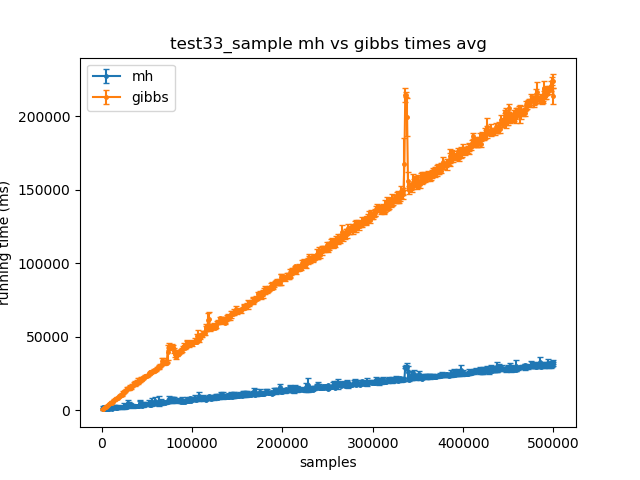
\includegraphics[width=1\textwidth]{plot_test33_sample_mh_vs_gibbs_times.png}
\caption{\label{fig:data}Comparison between MH and Gibbs methods.}
\end{figure}

Interpretation here.

\section{Discussion 1/2-1 page}
Discuss your results. Compare the two values of $n_{s}$ that you've found in the previous section. Compare your results with literature and comment on the difference. If you didn't know the value of the resistance quantum, would you be able to deduce it from your measurements? If yes/no, why?

\begin{thebibliography}{9}
\bibitem{nano3}
  K. Grove-Rasmussen og Jesper Nygård,
  \emph{Kvantefænomener i Nanosystemer}.
  Niels Bohr Institute \& Nano-Science Center, Københavns Universitet

\end{thebibliography}
\end{document}
